\documentclass[nooutcomes]{ximera}
%% handout
%% space
%% newpage
%% numbers
%% nooutcomes

%I added the commands here so that I would't have to keep looking them up
%\newcommand{\RR}{\mathbb R}
%\renewcommand{\d}{\,d}
%\newcommand{\dd}[2][]{\frac{d #1}{d #2}}
%\renewcommand{\l}{\ell}
%\newcommand{\ddx}{\frac{d}{dx}}
%\everymath{\displaystyle}
%\newcommand{\dfn}{\textbf}
%\newcommand{\eval}[1]{\bigg[ #1 \bigg]}

%\begin{image}
%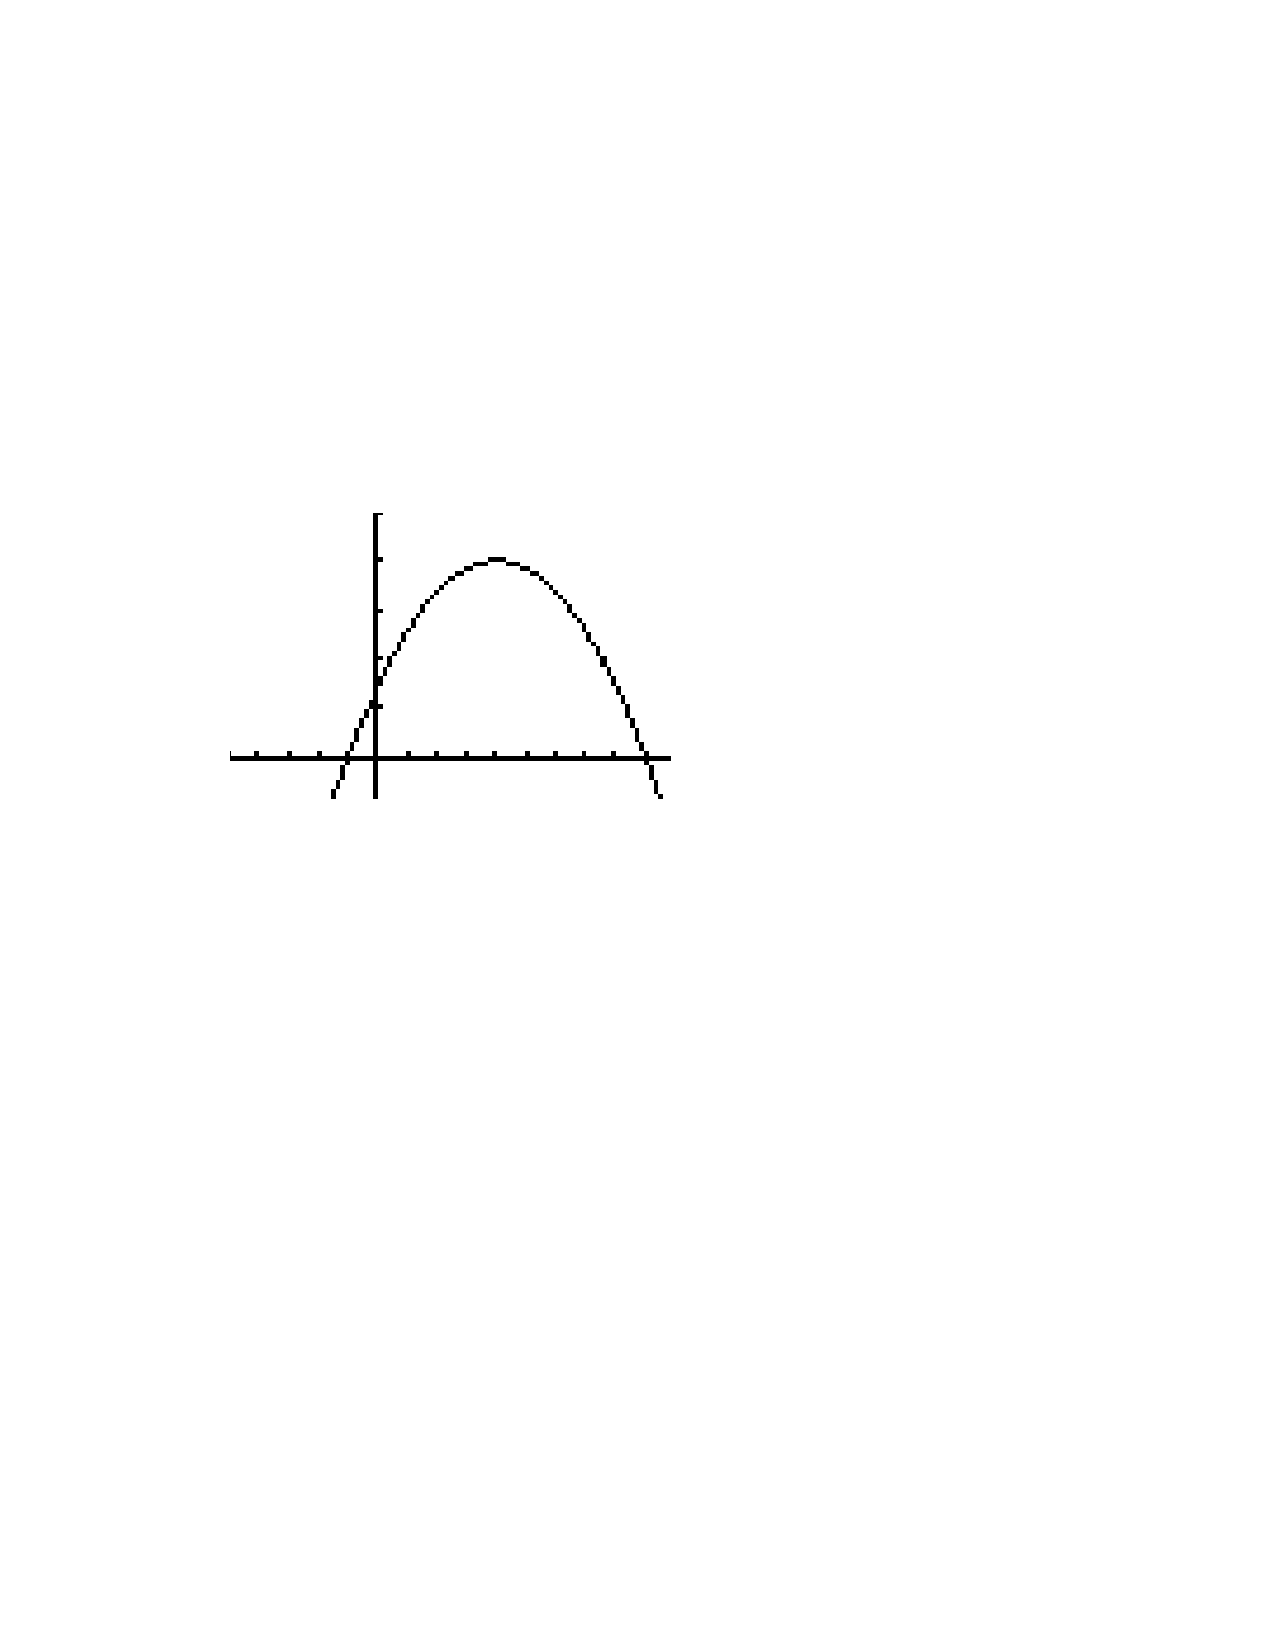
\includegraphics[trim= 170 420 250 180]{Figure1.pdf}
%\end{image}


\newcommand{\RR}{\mathbb R}
\renewcommand{\d}{\,d}
\newcommand{\dd}[2][]{\frac{d #1}{d #2}}
\renewcommand{\l}{\ell}
\newcommand{\ddx}{\frac{d}{dx}}
\newcommand{\dfn}{\textbf}
\newcommand{\eval}[1]{\bigg[ #1 \bigg]}

\usepackage{multicol}

\renewenvironment{freeResponse}{
\ifhandout\setbox0\vbox\bgroup\else
\begin{trivlist}\item[\hskip \labelsep\bfseries Solution:\hspace{2ex}]
\fi}
{\ifhandout\egroup\else
\end{trivlist}
\fi} %% we can turn off input when making a master document

\title{4.9 Antiderivatives (Solutions)}  

\begin{document}
\begin{abstract}		\end{abstract}
\maketitle

\section{Warm up:} 

		\begin{freeResponse}
		
		\end{freeResponse}	
		
		
		

	
	
	
	
	

\section{Group work:}



%problem 1
\begin{problem}
Find the most general antiderivative of the function
$$ g(t) = e^{-2t} - 5 + 6\sqrt{t}-\frac{7}{t} + \frac{5}{11 + t^2} $$
		\begin{freeResponse}
		Note that:
			\begin{itemize}
			\item  taking an antiderivative is \dfn{linear} over addition, meaning that we can find the antiderivative of each summand of $g(t)$, and then add them together.
			\item  An antiderivative of $e^{-2t}$ is $-\frac{1}{2} e^{-2t}$.
			\item  An antiderivative of $5$ is $5t$.
			\item  An antiderivative of $6 \sqrt{t}$ is $6 \left( \frac{2}{3} t^{\frac{3}{2}} \right) = 4t^{\frac{3}{2}}$.
			\item  An antiderivative of $\frac{7}{t}$ is $7 \ln |t|$.
			\item  An antiderivative of $\frac{5}{11 + t^2} = \frac{5}{11} \cdot \frac{1}{1 + \left( \frac{t}{\sqrt{11}} \right)^2 }$
			is $\frac{5}{\sqrt{11}} \arctan \left( \frac{t}{\sqrt{11}} \right)$
			\end{itemize}
		Thus, the most general antiderivative of $g(t)$ is:
		$$ -\frac{1}{2} e^{-2t} - 5t + 4t^{\frac{3}{2}} - 7 \ln |t| + \frac{5}{\sqrt{11}} \arctan \left( \frac{t}{\sqrt{11}} \right) + C $$
		\end{freeResponse}
		
		
\end{problem}
















%problem 2
\begin{problem}
Assume that $f^\prime (t) = 4t^3 + 2t$ and $f(3) = 5$.  Find $f(t)$.
		\begin{freeResponse}
		By taking the antiderivative of $f^\prime (t)$, we know that $f(t)$ is of the form
		$$f(t) = t^4 + t^2 + C .$$
		Then,
		$$ 5 = f(3) = 3^4 + 3^2 + C = 81 + 9 + C = 90 + C$$
		$$\Longrightarrow \quad  C = -85 $$
		and so
		$$ f(t) = t^4 + t^2 - 85. $$
		\end{freeResponse}
		
		
		

\end{problem}
	
	
	
	
	
	
	
	

		



	
	
	
	
	
	
	
	
	

	










								
				
				
	














\end{document} 


















